\documentclass[a4paper]{article}
\usepackage[english]{babel}
\usepackage[utf8]{vietnam}

%\usepackage{vntex}
\usepackage{listings} %chen code
\usepackage{float}
%\usepackage[english,vietnam]{babel}
%\usepackage[utf8]{inputenc}

%\usepackage[utf8]{inputenc}
%\usepackage[francais]{babel}
\usepackage{a4wide,amssymb,epsfig,latexsym,multicol,array,hhline,fancyhdr}

\usepackage{amsmath}
\usepackage{lastpage}
\usepackage[lined,boxed,commentsnumbered]{algorithm2e}
\usepackage{enumerate}
\usepackage{color}
\usepackage{graphicx}							
% Standard graphics package
\usepackage{array}
\usepackage{tabularx, caption}
\usepackage{multirow}
\usepackage{multicol}
\usepackage{rotating}
\usepackage{graphics}
\usepackage[a4paper,left=2cm,right=2cm,top=1.8cm,bottom=2.8cm]{geometry}
\usepackage{setspace}
\usepackage{epsfig}
\usepackage{tikz}
\usetikzlibrary{arrows,snakes,backgrounds}
\usepackage[unicode]{hyperref}
%can file puenc.def trong thu muc goc de option [unicode] tao ra bookmark bang tieng Viet
\hypersetup{urlcolor=blue,linkcolor=black,citecolor=black,colorlinks=true} 
%\usepackage{pstcol} 								
% PSTricks with the standard color package

\newtheorem{theorem}{{\bf Theorem}}
\newtheorem{property}{{\bf Property}}
\newtheorem{proposition}{{\bf Proposition}}
\newtheorem{corollary}[proposition]{{\bf Corollary}}
\newtheorem{lemma}[proposition]{{\bf Lemma}}


%\usepackage{fancyhdr}
\setlength{\headheight}{40pt}
\pagestyle{fancy}
\fancyhead{} % clear all header fields
\fancyhead[L]{
 \begin{tabular}{rl}
    \begin{picture}(25,15)(0,0)
    \put(0,-8){
\includegraphics[width=8mm, height=8mm]{hcmut.png}}
    %\put(0,-8){\epsfig{width=10mm,figure=hcmut.eps}}
   \end{picture}&
	%
\includegraphics[width=8mm, height=8mm]{hcmut.png} & %
	\begin{tabular}{l}
		\textbf{\bf \ttfamily Trường Đại Học Bách Khoa}\\
		\textbf{\bf \ttfamily Khoa Khoa Học \& Kỹ Thuật Máy Tính}
	\end{tabular} 	
 \end{tabular}
}
\fancyhead[R]{
	\begin{tabular}{l}
		\tiny \bf \\
		\tiny \bf 
	\end{tabular}  }
\fancyfoot{} % clear all footer fields
\fancyfoot[L]{\scriptsize \ttfamily Bài tập lớn - Mô Hình Hóa Toán Học, 2018-2019}
\fancyfoot[R]{\scriptsize \ttfamily Page {\thepage}/\pageref{LastPage}}
\renewcommand{\headrulewidth}{0.3pt}
\renewcommand{\footrulewidth}{0.3pt}


%%%
\setcounter{secnumdepth}{4}
\setcounter{tocdepth}{3}
\makeatletter
\newcounter {subsubsubsection}[subsubsection]
\renewcommand\thesubsubsubsection{\thesubsubsection .\@alph\c@subsubsubsection}
\newcommand\subsubsubsection{\@startsection{subsubsubsection}{4}{\z@}%
                                     {-3.25ex\@plus -1ex \@minus -.2ex}%
                                     {1.5ex \@plus .2ex}%
                                     {\normalfont\normalsize\bfseries}}
\newcommand*\l@subsubsubsection{\@dottedtocline{3}{10.0em}{4.1em}}
\newcommand*{\subsubsubsectionmark}[1]{}
\makeatother


\begin{document}

\begin{titlepage}

\begin{center}
TRƯỜNG ĐẠI HỌC BÁCH KHOA\\
KHOA KHOA HỌC \& KỸ THUẬT MÁY TÍNH
\end{center}

\vspace{1cm}

\begin{figure}[h!]
\begin{center}

\includegraphics[width=3cm]{hcmut.png}
\end{center}
\end{figure}

\vspace{1cm}


\begin{center}
\begin{tabular}{c}
\multicolumn{1}{l}{\textbf{{\Large MÔ HÌNH HÓA TOÁN HỌC}}}\\
~~\\
\hline
\\
\multicolumn{1}{l}{\textbf{{\Large Bài tập lớn}}}\\
\\
\textbf{\huge Xây dựng mô hình toán học để lựa chọn UTXO}\\
\\
\hline
\end{tabular}
\end{center}

\vspace{3cm}

\begin{table}[h]
\begin{tabular}{rrl}

\hspace{5 cm} & GVHD: Huỳnh Tường Nguyên & (htnguyen@hcmut.edu.vn)\\
& Lớp: L03-B & Nhóm: 12\\
& Thành viên nhóm: & Nguyễn Linh Đăng Minh - 1712177 \\
& & Cao Thành Nhân - 1710214 \\
& & Lương Thiện Chí - 1610304 \\
& & Trần Minh Tú - 1713850 \\
& & Trịnh Đức Thọ - 1713343 \\
& & Nguyễn Đình Thịnh - 1713325 \\
& & Phạm Văn Việt - 1713955 \\
\end{tabular}
\end{table}

\begin{center}
{\footnotesize Ho Chi Minh, 05/2019}
\end{center}
\end{titlepage}


%\thispagestyle{empty}
%\selectlanguage{english}
\newpage
\tableofcontents
\newpage


%%%%%%%%%%%%%%%%%%%%%%%%%%%%%%%%%
\section{Giới thiệu}

$\indent$\
Tiền mã hóa phi tập trung (decentralized cryptocurrency) là một tài sản kĩ thuật số sử dụng hệ thống mã hóa chọn lọc để đảm bảo an toàn cho giao dịch và tính minh bạch mà không cần sự tham gia can thiệp của bên thứ ba. Tất cả những giao dịch trong hệ thống đều được ghi lại trên một cuốn sổ cái (ledger) được gọi là blockchain - được cấu thành từ hàng loạt các khối khác nhau (block). Mỗi block chứa một con số không cố định của các giao dịch và đồng thời có một mã hash của block trước đó do đó tất cả các giao dịch trong blockchain rất khó để có thể thay đổi và trở nên hợp lệ vững chắc. Một ví dụ điển hình cho kiểu tiền mã hóa này chính là Bitcoin được giới thiệu vào năm 2008 mà hiện nay đang có hơn 141 tỉ USD trong thị trường tiền ảo, với 229 ngàn giao dịch và 183.89 GB lưu trữ trung bình trong một ngày. \\

Trong mỗi giao dịch dùng blockchains, thì chiến lược chọn UTXOs (Unspend Transaction Output set-Tập hợp các đầu ra giao dịch chưa chi tiêu) cho một giao dịch đóng một vai trò rất là quan trọng trong quản lí số dư tiền mã hóa của bất kì ví nào. Một chiến lược lựa chọn số tiền đã được tối ưu hóa thì phải thỏa mãn những ràng buộc cứng và những mục tiêu thiết yếu của ba nhóm chủ yếu như là users (người dùng), community (cộng đồng), và miners (người đào Bitcoin). Đứng từ phía người sử dụng, họ luôn muốn có thể tạo ra những giao dịch sẽ làm giảm thiểu phí giao dịch và đồng thời giữ được sự riêng tư của những giao dịch đó. Ngược lại, những miners lại tập trung vào khai thác những giao dịch có phí cao hơn càng nhiều càng tốt. Còn đối với cộng đồng, những UTXO cỡ lớn trở thành một vấn đề nan giải vì nó sẽ làm giảm thiểu hiệu suất xử lí các giao dịch và cũng sẽ gây ra những tiêu tốn chi phí lớn cho việc tiêu thụ bộ nhớ.\\

Trong phần nghiên cứu này, chúng tôi cân nhắc suy nghĩ về vấn đề chiến lược nghiên cứu để có thể chọn từ một tập các UTXOs đã được cho sẵn trong các giao dịch sao cho giảm được thấp nhất chí phí cho các miners hoặc tập hợp được càng nhiều các UTXO nhỏ để có thể giảm thiểu được kích thước của các UTXO.\\

Phần còn lại của báo cáo này được xây dựng theo các mục như sau: Mục 2. Xây dựng công thức cho vấn đề trình bày ngắn gọn nội dung và những yêu cầu của vấn đề đang được cân nhắc. Sau đó, chúng tôi trình bày những kết quả đạt được trong Mục 3. Đề xuất mô hình toán và Mục 4. Những suy lượng đã được hình thành từ việc thử nghiệm mô hình, và bàn luận về kết quả của việc thử nghiệm này. Cuối cùng, chúng tôi tổng hợp và đưa ra kết luận những kết quả của nhóm ở mục cuối cùng.  
\\	

%%%%%%%%%%%%%%%%%%%%%%%%%%%%%%%%%
\section{Xây dựng vấn đề}\label{fornul}
$\indent$\
Đối với một giao dịch nhất định, ví sẽ chọn một số UTXO từ tập UTXO sao cho có đủ giá trị để cấp vốn được gọi là giá trị mục tiêu. Lựa chọn tốt nhất là có một kết quả khớp chính xác với mục tiêu vì nó sẽ không sinh ra sự thay đổi đầu ra khi trả về cho người gửi để giảm thiểu kích thước giao dịch cũng như không làm cho kích thước tập UTXO bùng nổ. Sự thay đổi đầu ra là số lượng tiền còn lại sau khi cấp vốn và phải lớn hơn ngưỡng DUST (ngưỡng DUST là đầu ra của giao dịch trong đó phí để chuộc lại lớn hơn 1/3 giá trị của nó). Mục tiêu của DUST là ngăn chặn các giao dịch rác khi mà ai đó cố gắng làm suy giảm mạng bằng cách cố ý tạo ra các giao dịch rất nhỏ có thể tiêu tốn băng thông lớn. Ngoài ra, Bitcoin và các hệ thống tương tự khác hiện đang tính phí cho mỗi giao dịch để ngăn chặn các hành vi xấu và đảm bảo chỉ câc giao dịch hợp lệ dựa trên mạng blockchain.
\\

\\Mục tiêu của chúng ta là đề xuất một chiến lược hiệu quả trong việc lựa chọn một tập UTXO thích hợp cho một giao dịch nhất định, có khả năng đáp ứng nhiều ràng buộc sau:
\\1. Giảm thiểu kích thước giao dịch để có phí giao dịch tối thiểu.
\\2. Thu nhỏ tập UTXO.
\\

\\Điều đáng chú ý là nhận ra rằng đề xuất của chúng ta rõ ràng mang lại lợi ích cho người dùng và mục tiêu của cộng đồng. Thêm vào đó, chiến lược đề xuất của chúng ta muốn câc giao dịch được xác nhận nhanh nhất có thể bằng cách sử dụng mức phí phù hợp tùy thuộc vào nhu cầu của người sử dụng. Đây là một lợi ích ngầm cho các thợ mỏ.
\\
\\\textbf{Strategy 1 Proposed UTXO Selection}
\\\textbf{Objective} Xác định một tập hợp con của tập UTXO có giá cả phải chăng sao cho thỏa mãn ràng buộc cứng H1 và các ràng buộc mềm S1.
\\\textbf{Input} 
\\$\bullet$ U : Một tập của UTXOs.
\\$\bullet$ a : Số lượng đầu ra để gửi đến người nhận giao dịch.
\\$\bullet$ $\alpha$ : tỉ lệ phí khai thác.
\\$\bullet$ Các tham số khác được tóm tắt trong bảng 1.
\\\textbf{Output}
\\$\bullet$ Một tập hợp UTXO được chọn có thể chỉ chứa một output trùng khớp chính xác.
\\$\bullet$ Một đầu ra có thể thay đổi.
\\Ràng buộc cứng $H_1$
\\1. Một giao dịch phải có đủ giá trị để tiêu thụ.
\\2. Kích thước giao dịch không được vượt quá kích thước khối dữ liệu tối đa.
\\3. Tất cả các đầu ra giao dịch phải cao hơn ngưỡng DUST để chắc chắn rằng giao dịch này được chuyển tiếp đến mạng và được xác nhận.
\\Ràng buộc mềm $S_1$
\\1. Kích thước giao dịch được giảm thiểu.
\\2. Số lượng UTXO đã chọn được tối đa hóa để thu nhỏ kích thước nhóm UTXO.
\\
\\
\\
\begin{tabular}{|c|c|}
	\hline
	Input Parameters & Description \\ \hline
	U = $\{$$u_1$,...,$u_n$$\}$   & set of UTXOs   \\ \hline
	O = $\{$$o_1,...,o_n$$\}$   & set of transaction outputs   \\ \hline
	V^u = $\{$$v_1^u$,...,$v_n^u$$\}$   & set of UTXO's values   \\ \hline
	V^o = $\{$$v_1^o,...,v_n^o$$\}$   & set of transaction output's values   \\ \hline
	S^u = $\{$$s_1^u,...,s_n^u$$\}$   & set of transaction input size, with input is chosen from UTXO ui  \\ \hline
	S^o = $\{$$s_1^o,...,s_m^o$$\}$   & set of transaction output's size   \\ \hline
	M   & maximum size of a transaction   \\ \hline
	$\alpha$   & fee rate   \\ \hline
	T   & dust threshold   \\ \hline
	$\epsilon$   & minimum of change output   \\ \hline
\end{tabular}
\\
\begin{center}
	Bảng 1: CÁC THAM SỐ ĐẦU VÀO CỦA CÔNG VIỆC ĐÃ NÊU
\end{center}

%%%%%%%%%%%%%%%%%%%%%%%%%%%%%%%%%
\section{Đề xuất mô hình toán}\label{model}
$\indent$\ Sử dụng mô hình 2 để đưa ra chiến lược chọn UTXO dựa trên mô hình 1 như dưới đây: \\

\textbf{a) Mô hình 1:} \\\\
$\indent$\ - \textbf{Các biến:} \\
$\indent$\ + Biến quyết định: \\
\begin{center}
	$x_{i}= 
	\begin{cases}
	1, $	nếu UTXO được chọn$ \\ 
	0, $	ngược lại$
	\end{cases}
	$
\end{center}

+ Biến trung gian: \\
$\indent$\ \textbullet \ y: kích thước giao dịch \\
$\indent$\ \textbullet \  $z_{v}$: giá trị của đầu ra thay đổi \\
$\indent$\ \textbullet \  $z_{s}$: kích thước của đầu ra thay đổi \\
\begin{center}
	$z_{s}= 
	\begin{cases}
	0, $	0 $\le$ $z_{v}$ $\le$ $\epsilon$ $ \\
	\beta, $ $z_{v}$ > $\epsilon$	 $ \\
	\end{cases}
	$
\end{center}
$\indent$\ \textbf{- Các ràng buộc:} \\
$\indent$\ \textbullet \ Kích thước giao dịch không được vượt quá kích thước dữ liệu khối tối đa. \\
\begin{center}
	y = $\sum\limits_{i|u_{i} \in U}^{}$ $s^{u}_{i}$*$x_{i}$ + $\sum\limits_{j|o_{j} \in O}^{}$ $s^{o}_{j}$+$z_{s}$ $\le$ M
\end{center}
$\indent$\ \textbullet \ Một giao dịch phải có đủ giá trị để tiêu thụ. \\
\begin{center}
	$\sum\limits_{i|u_{i} \in U}^{}$ $v^{u}_{i}$*$x_{i}$ = $\sum\limits_{j|o_{j} \in O}^{}$ $v^{o}_{j}$+$\alpha$*y+$z_{v}$
\end{center}
$\indent$\ \textbullet \ Tất cả các đầu ra giao dịch phải cao hơn ngưỡng bụi để chắc chắn rằng giao dịch này được chuyển tiếp đến mạng và được xác nhận. \\
\begin{center}
	T $\le$ $\sum\limits_{j|o_{j} \in O}^{} v^{o}_{j} $
\end{center}
$\indent$\ \textbullet \ Mối quan hệ giữa  giá trị đầu ra thay đổi $z_{v}$ và kích thước của nó $z_{s}$ được định nghĩa như sau:\\
\begin{center}
	$z_{s} \le  	\Bigl\lfloor\dfrac{z_{v}}{\epsilon}\Bigr\rfloor\ * \beta $
	
\end{center}
$\indent$\ \textbullet \ $x_{i}$ là biến nhị phân. \\
\begin{center}
	$ \forall i|u_{i} \in U : x_{i} \in \left\{0,1\right\} $
\end{center}

\textbf{- Hàm mục tiêu:} Giảm thiểu kích thước giao dịch \\
\begin{center}
	minimize y
\end{center}
$\indent$\ \textbf{ b) Mô hình 2: được xây dựng dựa trên kết quả thu được của mô hình 1} \\\\
$\indent$\ \textbf{- Các biến:}  Bao gồm tất cả các biến của mô hình 1. \\
$\indent$\ \textbf{- Các ràng buộc:} Bao gồm tất cả các ràng buộc của mô hình 1 và bổ sung thêm ràng buộc sau: 
\begin{center}
	$ y < (1 + \gamma) \times Y $, trong đó
\end{center}
$\indent$\ \textbullet \ Y là kích thước giao dịch tối thiểu thu được từ Mô hình 1. \\
$\indent$\ \textbullet \ $\gamma$ là hằng số (0 < $\gamma$ < 1). \\
$\indent$\ \ Nếu $\gamma$ gần về 0, ta giữ kích thước giao dịch tối thiểu thu được từ Mô hình 1. Mặt khác, giao dịch có kích thước phù hợp được tạo bởi một số UTXO càng lớn càng tốt. \\
$\indent$\ \textbf{- Hàm mục tiêu:} Tối đa hóa số lượng UTXO.
\begin{center}
	maximize ($\sum\limits_{i|u_{i} \in U}^{} x_{i} - z_{s} / \beta $)
\end{center}

%%%%%%%%%%%%%%%%%%%%%%%%%%%%%%%%%
\section{Đánh giá những kết quả đã được hiện thực}\label{eval}

$\indent$\textcolor{red}{Input format:}

Tập dữ liệu bao gồm 133 file data định dạng .dat tương ứng với 133 trường hợp địa chỉ chứa các UTXOs đang khảo sát. Quan sát tập dữ liệu sẽ giúp ta hiểu rõ hơn về việc các UTXOs được chọn trong mạng lưới như thế nào. Tập dữ liệu bao gồm 133 trường hợp, trong đó không có địa chỉ nào có 1 hoặc không có UTXOs; có 99 địa chỉ chứa từ 2 đến 10 UTXOs trong tổng số 133 địa chỉ, chiếm tỉ lệ cao nhất(75\%); có 19 trường hợp có từ 11 đến 100 UTXOs (chiếm khoảng 14.39\% tổng thể) và 14 trường hợp có từ 101 đến 100000 UTXOs (khoảng 10.61\% tổng thể). Figure 1 thể hiện rõ phân bố tần suất của các UTXOs trong các địa chỉ.

\newpage
\begin{center}
	\begin{figure} []
		\begin{center}
			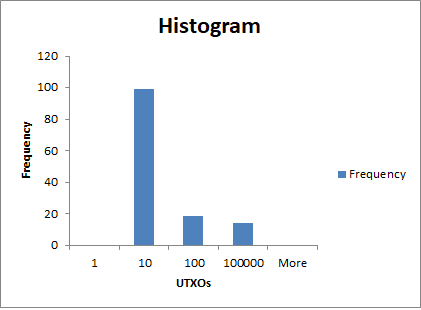
\includegraphics[scale=1]{tansuatUTXOs}
		\end{center}
		\caption{Tần suất UTXOs trong các địa chỉ}
		\label{refhinh1}
	\end{figure}
\end{center}

<Cấu trúc file "dat.dat">
\begin{lstlisting}[frame=single]

/*********************************************
* OPL 12.9.0.0 Data
* Author: Tanaka Kai
* Creation Date: May 5, 2019 at 2:39:14 PM
*********************************************/
datFiles = {"5ad448a959678302d59e6f75",
"5ad44bfdce94cf05c955f862",
"5ad44e0ece94cf05c955f864",
"5ad44e1bce94cf05c955f865",
.......
.......
.......			
"5ad4c6024c372215dd13d6bd",
"5ad4cb594c372215dd13d6be",
"5ad4cb834c372215dd13d6bf"};

\end{lstlisting}


<Cấu trúc 1 file dữ liêu "[ID].dat">
\begin{lstlisting}[frame=single]

input = <
2, 
1, 
61480, 
1048576, 
1.38313609467456, 
756, 
756, 
34, 
1352, 
330, 
0, 
0, 
>;

UTXOs = { 
<1, 148, 30234>, 
<2, 148, 33116>, 
};

output = { 
<1, 34, 61480>, 
};

\end{lstlisting}

\textcolor{red}{Output format:}

Sau khi xử lí bằng IBM CPLEX Optimization Studio 12.9.0, kết quả được đưa về dạng file csv để thuận tiện cho việc xử lý sau này.

\begin{center}
	\begin{figure} [ht]
		\begin{center}
			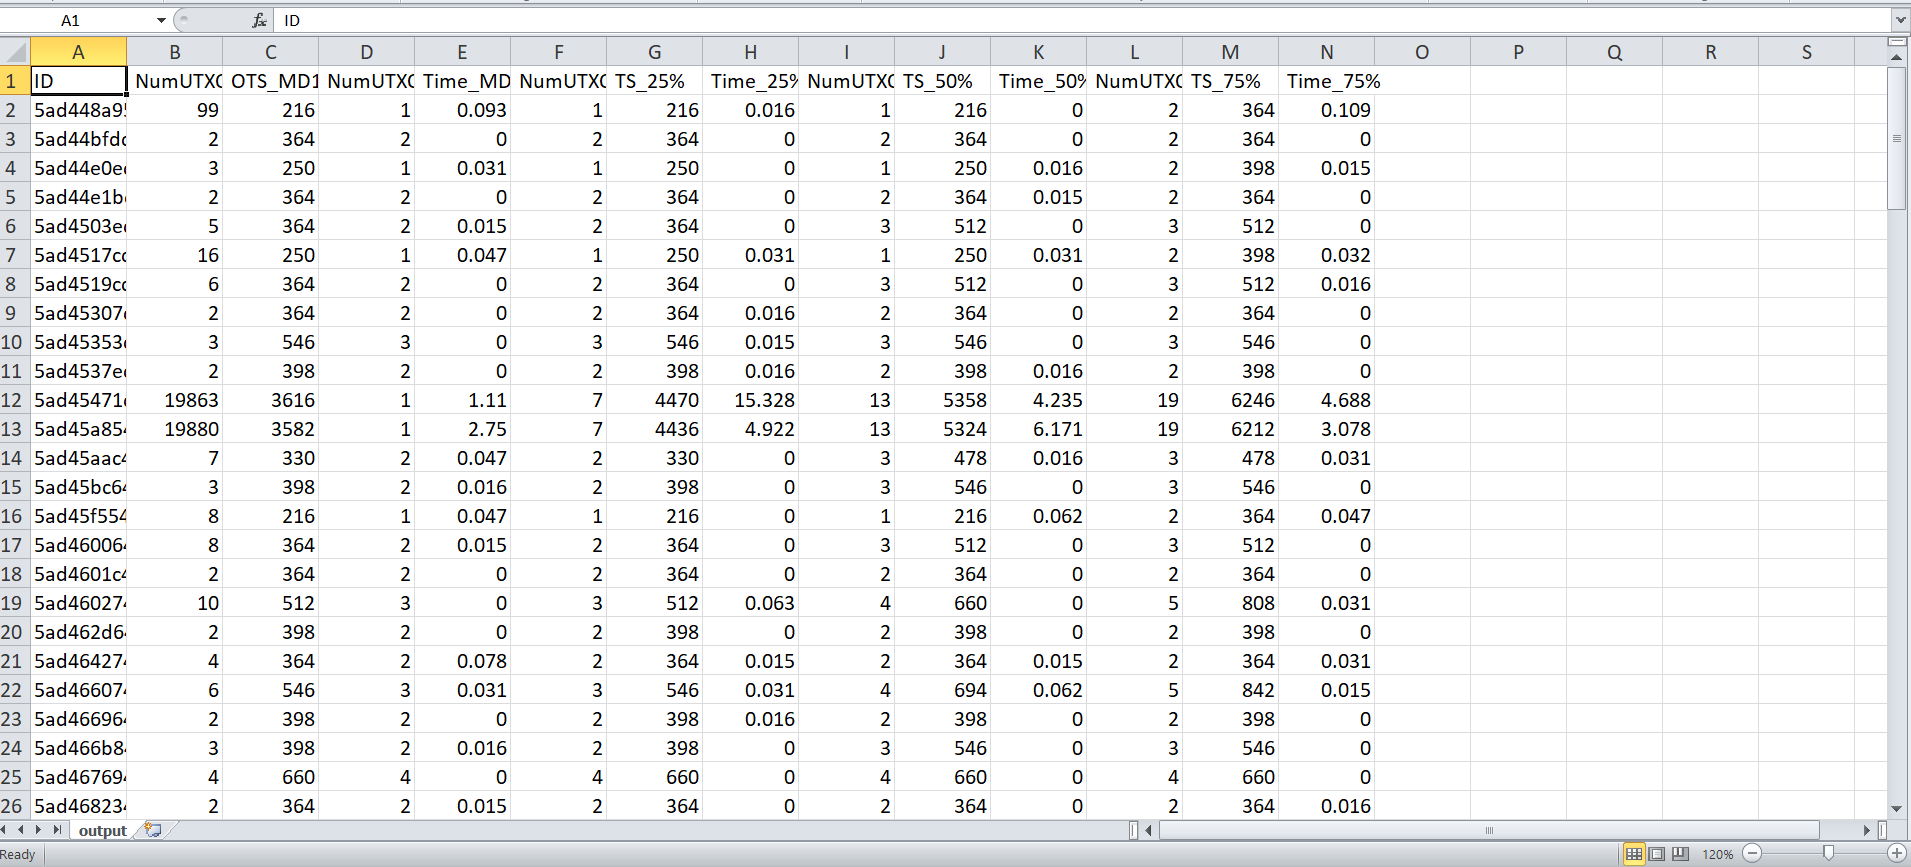
\includegraphics[scale=.43]{output}
		\end{center}
		\caption{Output format}
		\label{refhinh1}
	\end{figure}
\end{center}

\textcolor{red}{Implementation in GLPK/AMPL:} IBM CPLEX Optimization Studio 12.9.0

<File "sub.mod">
\begin{lstlisting}[frame=single]

tuple vin {
int vid;
int vsize;
int vValue; 
}

tuple vout {
int vid;
int vsize;
int vValue; 
}

tuple inputSet {
int n;
int m;
float outValue;
float M;
float alpha;
float T;
float epsilon;
int beta;
int txsize;
int iosize;
float cout;
float coutValue;
}

inputSet input = ...;

{vin} UTXOs = ...;

{vout} output = ...;

int outputSize = sum(e in output) e.vsize;

dvar boolean a[UTXOs];
dvar int+ zsize;
/*range n = 1..input.n;*/
//dexpr float minv=min(forall(e in UTXOs, a[e] diff 0)) a[e]*e.vsize;
dexpr int inputSize = sum(e in UTXOs) a[e]*e.vsize;
dexpr int inputValue = sum(e in UTXOs) a[e]*e.vValue;

dexpr int transactionSize = inputSize + outputSize + zsize;
dexpr float zvalue = inputValue - (input.outValue + input.alpha*transactionSize);
minimize transactionSize;

subject to {
cons0:
(zvalue <= input.epsilon - 0.0001) => (zsize == 0);
(zvalue >= input.epsilon) => (zsize == input.beta);
cons1:
inputSize + outputSize + zsize <= input.M;
cons2: 
forall (out in output)
out.vValue >= input.T;
cons3:
zvalue >= 0;
}

int numUTXO = sum(e in UTXOs) a[e];

execute {
writeln(numUTXO);
}

\end{lstlisting}



<File "mainflow.mod">
\begin{lstlisting}[frame=single]

{string} datFiles = ...;

float k = ...;

float Y = ...;

main {
var file = new IloOplOutputFile("output.txt"); 
file.writeln("ID, NumUTXO, OTS_MD1, NumUTXOUsed_MD1, Time_MD1, NumUTXOUsed_25%, TS_25%, Time_25%, NumUTXOUsed_50%, TS_50%, Time_50%, NumUTXOUsed_75%, TS_75%, Time_75%")

var source = new IloOplModelSource("sub.mod");
var cplex = new IloCplex();
var def = new IloOplModelDefinition(source);

for (var datFile in thisOplModel.datFiles) { 	

var opl = new IloOplModel(def, cplex);
var data = new IloOplDataSource(datFile+".dat");
opl.addDataSource(data);
opl.generate();
if (cplex.solve()) {
opl.postProcess();

file.write(datFile+", ");
file.write(opl.input.n+", ");
file.write(cplex.getObjValue()+", ");
file.write(opl.numUTXO+", ");
file.write(cplex.getSolvedTime()+", ");

var optValue = cplex.getObjValue();
writeln("OBJ = "+ cplex.getObjValue());

//k = 0,25
var source2 = new IloOplModelSource("sub_2.mod");
var cplex = new IloCplex();
var def2 = new IloOplModelDefinition(source2);
var opl2 = new IloOplModel(def2, cplex);
var data2 = new IloOplDataElements();
data2.k = 0.25;
data2.Y = optValue;
opl2.addDataSource(data);
opl2.addDataSource(data2);

opl2.generate();

if (cplex.solve()) {
file.write(opl2.selected+", ");
file.write(opl2.transactionSize+", ");
file.write(cplex.getSolvedTime()+", ");
}
else {
writeln("No solution") 			
}

//k = 0.5
var source2 = new IloOplModelSource("sub_2.mod");
var cplex = new IloCplex();
var def2 = new IloOplModelDefinition(source2);
var opl2 = new IloOplModel(def2, cplex);
var data2 = new IloOplDataElements();
data2.k = 0.5;
data2.Y = optValue;
opl2.addDataSource(data);
opl2.addDataSource(data2);

opl2.generate();

if (cplex.solve()) {
file.write(opl2.selected+", ");
file.write(opl2.transactionSize+", ");
file.write(cplex.getSolvedTime()+", ");
}
else {
writeln("No solution") 			
}

//k = 0.75
var source2 = new IloOplModelSource("sub_2.mod");
var cplex = new IloCplex();
var def2 = new IloOplModelDefinition(source2);
var opl2 = new IloOplModel(def2, cplex);
var data2 = new IloOplDataElements();
data2.k = 0.75;
data2.Y = optValue;
opl2.addDataSource(data);
opl2.addDataSource(data2);

opl2.generate();

if (cplex.solve()) {
file.write(opl2.selected+", ");
file.write(opl2.transactionSize+", ");
file.writeln(cplex.getSolvedTime()+", ");
}
else {
writeln("No solution") 			
}
}	
else {
writeln("No solution"); 		
}
opl.end();
} 
}
\end{lstlisting}



\textcolor{red}{Experimental results}

Mô hình đã đề xuất được giải bởi IBM CPLEX Studio Optimization 12.9.0. Giá trị của $\gamma$ trong Model 2 được thực nghiệm lần lượt là 25\%, 50\%, 75\%. Kết quả lấy được sẽ được so sánh với kết quả sẵn có của các phương pháp HVF, LVF, OF.

\begin{table}[ht]
	\begin{tabular}{|l|l|l|l|l|l|l|l|}
		\hline
		Method     & HVF    & LVF     & OF     & Model 1 & Model 2($\gamma$=25\%) & Model 2($\gamma$=50\%) & Model 2($\gamma$=75\%) \\ \hline
		NoSelected & 330.00 & 1361.00 & 855.00 & 315.00  & 373.00        & 469.00        & 559.00        \\ \hline
	\end{tabular}
\end{table}

\begin{center}
	\begin{figure} [ht]
		\begin{center}
			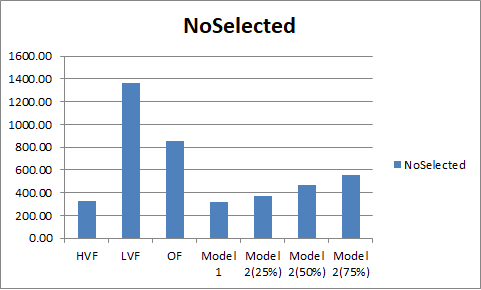
\includegraphics[scale=1]{NoSelected}
		\end{center}
		\caption{Số lượng UTXOs được chọn ở mỗi phương pháp}
		\label{refhinh1}
	\end{figure}
\end{center}

Đối với Model 1, số lượng UTXOs được chọn rất ít, tổng cộng chỉ có 315 cái được chọn, thấp hơn cả mô hình HVF. Model 2 với các giá trị $\gamma$ được khảo sát cho kết quả UTXOs được chọn nhiều hơn nhưng vẫn ở mức thấp, chưa bằng mô hình OF và thấp hơn nhiều so với mô hình LVF.

\begin{table}[ht]
	\begin{tabular}{|l|l|l|l|l|l|l|l|}
		\hline
		Method  & HVF & LVF & OF & Model 1 & Model 2($\gamma$=25\%) & Model 2($\gamma$=50\%) & Model 2($\gamma$=75\%) \\ \hline
		RunTime & 69  & 79  & 62 & 13.234  & 74.622        & 81.703        & 52.393        \\ \hline
	\end{tabular}
\end{table}

\begin{center}
	\begin{figure} [ht]
		\begin{center}
			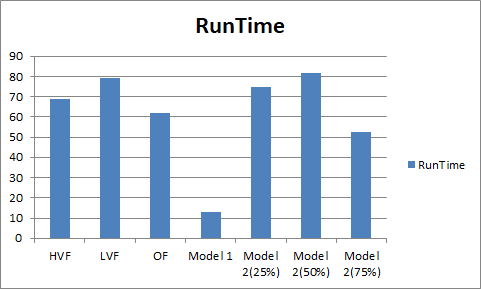
\includegraphics[scale=1]{RunTime}
		\end{center}
		\caption{Thời gian chạy giải thuật của mỗi phương pháp}
		\label{refhinh1}
	\end{figure}
\end{center}

Từ những số liệu thống kê trên, ta có thể thấy Model 1 tốn rất ít thời gian sô với các mô hình còn lại( chỉ xấp xỉ 13.234s). Trong khi đó, Model 2 cho kết quả thời gian chạy khá tương đồng với các mô hình HVF, LVF, OF.

\begin{table}[ht]
	\begin{tabular}{|l|l|l|l|l|l|l|l|}
		\hline
		Method  & HVF & LVF & OF & Model 1 & Model 2($\gamma$=25\%) & Model 2($\gamma$=50\%) & Model 2($\gamma$=75\%) \\ \hline
		TransactionSize & 399724 & 551632 & 477526 & 85618   & 93794         & 107900        & 121152        \\ \hline
	\end{tabular}
\end{table}

\begin{center}
	\begin{figure}[!ht]
		\begin{center}
			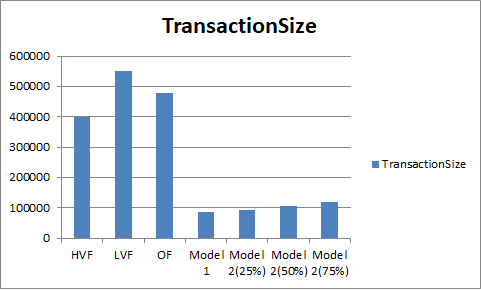
\includegraphics[scale=1]{TransactionSize}
		\end{center}
		\caption{Tổng kích thước giao dịch của mỗi phương pháp}
		\label{refhinh1}
	\end{figure}
\end{center}

Kích thước giao dịch của các Model 1 và 2 là khá nhỏ và thấp hơn nhiều so với các mô hình HVF, LVF, OF.\\

Từ những số liệu trên, ta có thể thấy mô hình 1 tuy có thời gian chạy rất thấp nhưng số lượng UTXOs được chọn cũng rất thấp. Trong khi đó, ở mô hình 2, với những giá trị $\gamma$ để kiểm soát lần lượt là 25\%, 50\%, 75\%, ta có thể thấy thời gian chạy vẫn được giữ xấp xỉ với các mô hình HVF, LVF, OF, nhưng số lượng UTXOs được chọn đã được tăng lên đáng kể, đồng thời kích thước giao dịch vẫn tương đối ổn định so với mô hình 1.

%%%%%%%%%%%%%%%%%%%%%%%%%%%%%%%%%
\newpage
\section{Conclusion}
$\indent$
Trong bài báo cáo này, nhóm chúng tôi đã hiện thực hai mô hình đã đưa ra để đánh giá về việc giải quyết hai mục tiêu thiết yếu khi tạo giao dịch mới trên blockchain. Đó là giảm thiểu kích thước giao dịch để có phí giao dịch tối thiểu và thu nhỏ tập UTXO. Mô hình 1 tối thiểu được kích thước giao dịch tuy nhiên không giải quyết được nhu cầu thu nhỏ tập UTXO nên chúng tôi đưa ra mô hình 2 để giải quyết được cả 2 vấn đề này. Mô hình 2 được đưa ra để vừa có thể chọn được càng nhiều UTXO càng tốt nhưng không làm cho kích thước giao dịch quá lớn, do chúng tôi đã kiểm soát bằng tỉ lệ gamma nên luôn đảm bảo kích thước giao dịch không lớn quá mức cho phép làm tăng phí giao dịch. Qua đó ta có thể thấy được so với các mô hình hiện tại là HVF và LVF thì rõ ràng mô hình trên hiệu quả hơn. Mặc dù cần được thử nghiệm với các tập dữ liệu lớn hơn nữa nhưng rõ ràng mô hình đã đưa ra hoàn toàn khả thi để đưa vào thực tế.

\newpage
%%%%%%%%%%%%%%%%%%%%%%%%%%%%%%%%%

\begin{thebibliography}{80}
	
	
	\bibitem{http://wikipedia:2015} wikipedia.
	``\textbf{link: http://en.wikipedia.org/}'',
	\textit{}, last access: 05/05/2015.
	
	
	\bibitem{Frey2016}	Frey, D., Makkes, M. X., Roman, P.-L., Taiani,  F.,  Voulgaris, S.: Bringing secure Bitcoin transactions to your smartphone. The 15th International Workshop on Adaptive and Reflective Middleware, (2016).
	
	\bibitem{Andreas2014} Antonopoulos, A. M.: Mastering Bitcoin. 2nd edn. O'Reilly Media, CA 95472 (2014).
	
	\bibitem{Bitcoinjs} Bitcoinjs: Open Source Organisation for Bitcoin JavaScript Libraries,https://github.com/bitcoinjs. Last accessed 15 August 2018.
	
	\bibitem{Bitcoinj}	Bitcoinj: Library for working with the Bitcoin protocol,https://bitcoinj.github.io. Last accessed 10 August 2018.
	
	\bibitem{Yanovich:2016} Yanovich, Y., Mischenko, P.,  Ostrovskiy,  A.:  Shared Send Untangling in Bitcoin, White paper, Bitfury Group Limited (2016).
	
	\bibitem{Patrick-Dai:2016} Dai, P., Mahi, N., Earls, J., Norta, A.: Smart-Contract Value-Transfer Protocols on a Distributed Mobile Application Platform,  https://qtum. org/uploads/files/cf6d69348ca50dd985b60425ccf282f3.pdf, (2016).
	
	\bibitem{Sergi:2017} Sergi, D.-S., Cristina, P.-S., Guillermo, N.-A., Jordi, H.-J.: Analysis of the Bitcoin UTXO set, IACR Cryptology ePrint Archive, (2017).
	
	\bibitem{Mark-Erhardt:2016} Erhardt, M.: An Evaluation of Coin Selection
	Strategies, Master thesis, Karlsruhe Institute of Technology, URL: http://murch.one/wp-content/uploads/2016/11/erhardt2016coinselection.pdf, (2016).
	
	\bibitem{Zahnentferner:2018} Zahnentferner, J.: Chimeric ledgers: Translating and unifying utxo-based and account-based cryptocurrencies, Cryptology ePrint Archive, Report 2018/262, 2018. https://epri nt. iacr. org/2018/262, (2018).
	
	\bibitem{Chepurnoy:2018} Chepurnoy, A., Kharin, V., Meshkov, D.: A Systematic Approach To Cryptocurrency Fees. IACR Cryptology ePrint Archive, (2018).
\end{thebibliography}
\end{document}
	
	\bibitem{Yanovich:2016} Yanovich, Y., Mischenko, P.,  Ostrovskiy,  A.:  Shared Send Untangling in Bitcoin, White paper, Bitfury Group Limited (2016).
	
	\bibitem{Patrick-Dai:2016} Dai, P., Mahi, N., Earls, J., Norta, A.: Smart-Contract Value-Transfer Protocols on a Distributed Mobile Application Platform,  https://qtum. org/uploads/files/cf6d69348ca50dd985b60425ccf282f3.pdf, (2016).
	
	\bibitem{Sergi:2017} Sergi, D.-S., Cristina, P.-S., Guillermo, N.-A., Jordi, H.-J.: Analysis of the Bitcoin UTXO set, IACR Cryptology ePrint Archive, (2017).
	
	\bibitem{Mark-Erhardt:2016} Erhardt, M.: An Evaluation of Coin Selection
	Strategies, Master thesis, Karlsruhe Institute of Technology, URL: http://murch.one/wp-content/uploads/2016/11/erhardt2016coinselection.pdf, (2016).
	
	\bibitem{Zahnentferner:2018} Zahnentferner, J.: Chimeric ledgers: Translating and unifying utxo-based and account-based cryptocurrencies, Cryptology ePrint Archive, Report 2018/262, 2018. https://epri nt. iacr. org/2018/262, (2018).
	
	\bibitem{Chepurnoy:2018} Chepurnoy, A., Kharin, V., Meshkov, D.: A Systematic Approach To Cryptocurrency Fees. IACR Cryptology ePrint Archive, (2018).
\end{thebibliography}
\end{document}

